% \section{Abstract}

\section{Introduction}

The imbalance between compute and memory capacity for data
center servers has only increased over the past decade.
Simultaneously networks have doubled in capacity at an
increasing rate and have integrated line rate
programmability into many commodity chips. These trends have
yielded various research proposals for attacking the
\textit{memory wall} with fast networks. Memory
disaggregation proposes the addition of pools of far-memory
attached over a network to clusters of compute machines,
with the promise that large shared pools will decrease
memory stranding and increase overall memory utilization.

Latency is the chief challenge in realizing practical memory
disaggregation. Low-latency interconnects such as RDMA have
intra-rack round trip latencies on the order of 1-2$\mu$s.
In contrast to local memory DRAM access times of 50-100ns
RDMA latency is a 20x overhead. This disparity prevents many
data structures, and system functions from being deployable
for remote memory. Existing systems have amortized the
network cost by porting slower subsystems i.e swap devices
~\cite{fastswap, legoos}\todo{add more}. 

These systems avoid a key feature of local memory
\textit{sharing}. Shared data structures in remote memory
can suffer abysmal performance when accessed concurrently.
Both traditional lock based and optimistically concurrent
data structures suffer abysmal performance when ported to
remote memory. Lock based algorithms have inflated critical
section sizes due to round trip delays, and optimistic
approaches suffer from stale caches under contention, and
the increased cost of reading to synchronize caches. In
general shared structures are hard to port to remote memory.

%% Todo this is my research statement work hard on it.
My work focuses on the design of algorithms and data
structures for remote memory.  A key insight of my work is
that the performance pitfalls of remote memory arise from
memory not having colocated compute to serialize operations.
We note that this pitfall is unnecessary because the network
implicitly serializes each operation during transit and
programable elements within the network can administrate
algorithm level serialization at line rate. With this
observation in mind we design shared far memory systems
using programmable devices such as NIC's and switches to
accelerate performance.

This research summary covers three projects which illustrate
how these devices can be used to improve optimistic data
structures, lock-based structures, and finally, shared
structures in general.  The first system \textit{Swordbox}
demonstrates that by caching the operations of an optimistic
algorithm on a programmable switch contention can be
entirely removed in network enabling up to 40x improvement
in throughput and 300x reduction in tail latency for
contested workloads. The second project \textit{RCuckoo}
shows how with careful algorithm design and the judicial use
of RDMA features a traditional local memory algorithm can be
ported to remote memory. Finally this work presents an
outline for general data structure design for remote memory
using a programmable switch to remove contention in the
general case.


\section{Optimistic Data Structures}

Optimistic concurrency enables high degrees of parallelism
in the absence of contention. At a high level concurrent
processes keep a cache of a shared structures state, and
then issue operations which succeed if the cache of read, or
written data is synchronized with the shared structure. When
memory latency, and contention are high synchronization is
difficult as reads are slower and more expensive quickly
causing local caches to become stale.

In our work \textit{Swordbox} we make the observation that
at rack-scale the top-of-rack (TOR) switch observes all
memory operations in serialized order. This de facto
serialization enables a programmable switch to resolve
conflicting updates to a shared data structure in flight.

In our prototype we resolve optimistic updates to a shared
link list which underpins Clover, a state of the art
disaggregated key value store~\cite{clover}. In Clover keys
are stored as a linked list, when clients update a key they
issue an append to the tail of the list. When keys are under
contention appends to the list frequently fail as the
clients issue appends to stale version of the lists' tail.

Figure~\ref{fig:swordbox} a) shows how the success rate of
clovers writes plummets as the number of concurrent clients
increase. When requests fail, clients must issue reads to
the list, find the tail, and execute the write again causing
throughput to drop, and tail latency to dramatically
increase. Swordbox fixes this performance pitfall by caching
the tail pointer of hot keys in a P4 program running on a
programmable TOR. When write pass through Swordbox it
updates it's tail pointer to the list.  When Swordbox sees
stale writes, i.e writes issued to old tail locations, it
rewrites the virtual address of the write to append it to
the tail of the list. This technique enables all contested
request to succeed while using only a small amount of switch
SRAM (64bits per key). Figure~\ref{fig:swordbox} b,c shows
both the throughput (32x) and latency (300x) improvements of
using Swordbox.

Swordbox demonstrates that optimistic algorithms can be
dramatically improved by caching contested variables in
network. Data structures which require updates to many
locations within a structure may be less amenable to
swordbox's design as the amount of state required to perform
the updates may be large. The future direction for this work
is to investigate data structure design which enables large
performance boosts through small amounts of in-network
caching.

\begin{figure*}[t!]
    \begin{subfigure}{.33\textwidth}
      \centering
      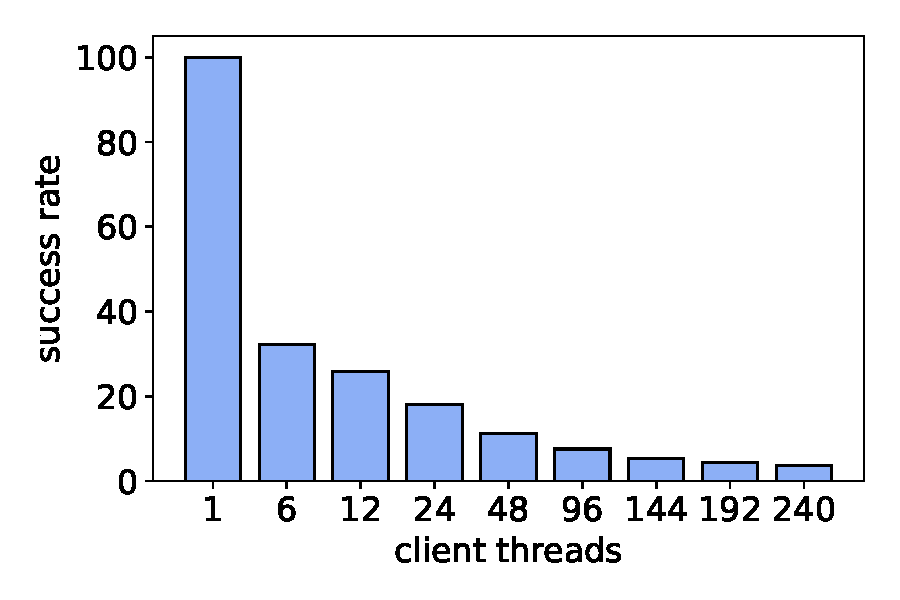
\includegraphics[width=.9\linewidth]{fig/success_rate.pdf}
    \end{subfigure}%
    \begin{subfigure}{.33\textwidth}
      \centering
      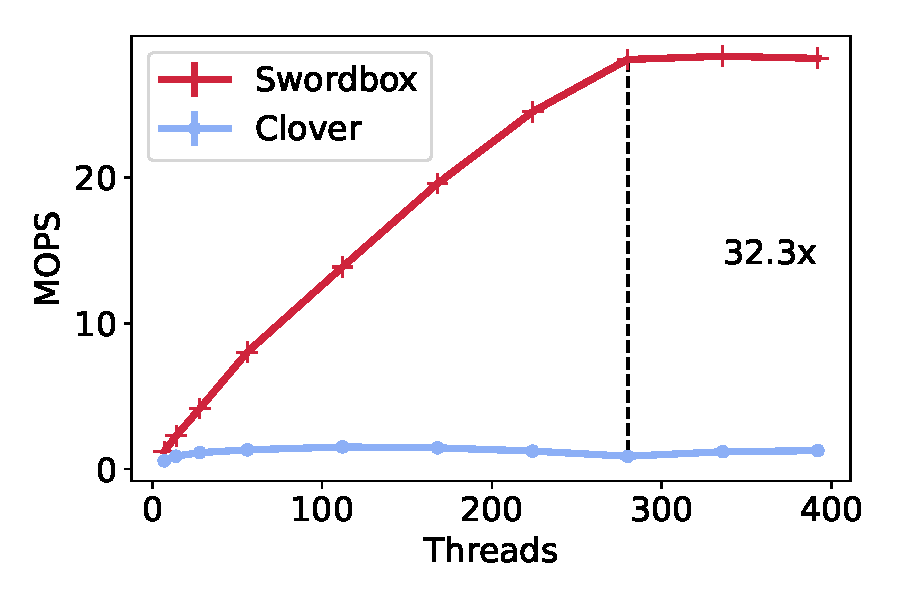
\includegraphics[width=.9\linewidth]{fig/full_system_performance.pdf}
    \end{subfigure}
    \begin{subfigure}{.33\textwidth}
      \centering
      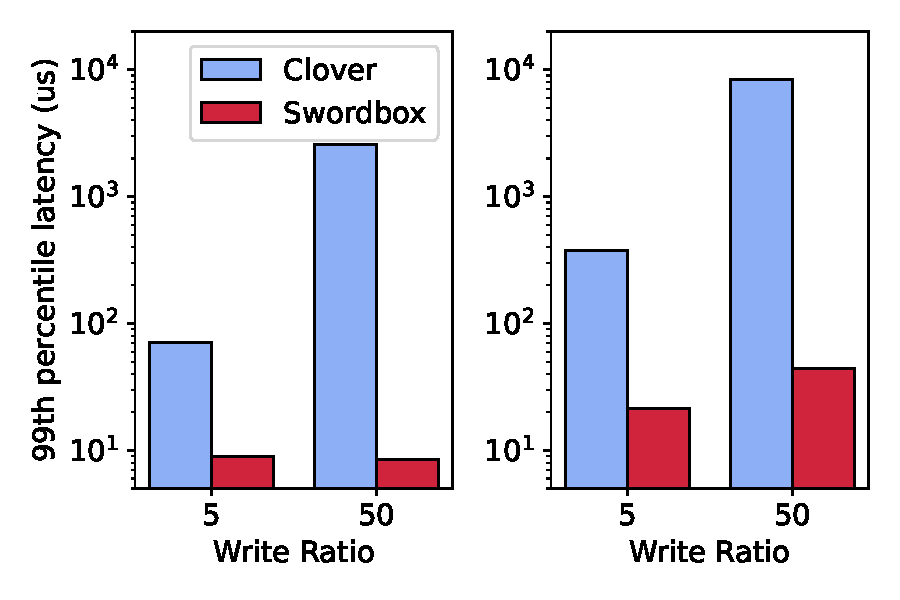
\includegraphics[width=.9\linewidth]{fig/99th_latency.pdf}
    \end{subfigure}

    \caption{Swordbox performance benifits. \textbf{a)} The effect of contention on
    Clover's optimistic writes. \textbf{b)} System throughput
    for YCSB-A (50\% write). \textbf{c)} 99th percentile tail
    latency for different write percentages. Left: read
    latency. Right: write latency}
        
    \label{fig:swordbox}
\end{figure*}

\section{RCuckoo}

Not all data structures are amenable to oportunistic
updates, but traditional locking port poorly to remote
memory. Acquiring, and then releasing a lock requires at
minimum two round trips, a fact which not only increases the
minimum operation duration, but which sets a minimum
duration on critical sections. A system with a 2us round
trip time, and a single global lock can only perform 500,000
operations per second in the best case (meger numbers when
considering that decakes old key value stores acheive 10's
of millions of requests per second ~\cite{herd}). Fine
grained locking is a requirement. Unfortunatly fine grained
locking suffers from a duel problem, deadlock free lock
acquisition requires a round trip per lock inflating
operation time. 

With RDMA atomics many locks can be aquired in a single
operation, but only if they are within the word width of the
RDMA atomic (64 bits). Fine grained locking is therefore a
challenge of achieving good lock locality.

With this in mind we investigate porting cuckoo hashing to
remote memory. Cuckoo hashing has long been known to perform
well with RDMA reads as lookups must search at most 2
locations~\cite{pilaf, farm}. The complexity of cuckoo
hashing is pushed to writes which perform swaps randomly
throughout the table. We develop a new algorithm for
locality aware cuckoo hashing. Both hash location are with
high probabiltiy located close together. Insertions are
therefore more likely to be localized to a small reigion of
the tabe rather than random, and the locks can be aquired in
few round trips. In addition we use locality to improve
searching for hash table openings using locality aware
search (A*) to find minimal distance insertion paths. We
achieve on average 2 round trips per insertion and
demonstrate that we out perform state of the art remote
memory hashing algorithms in simulation.

\todo{add the figure of the A* search and the number of
round trips per lock}


\section{Black Box Disaggregation}

A question remains about general data structure design for
remote memory. while high performanc can be achieved through
careful data structure design, is it possible enable general
data structure design for remote memory? My future research
direction aims to explore this question.

Prior work on NUMA systems has shown that highly concurrent
data structures can be desigend in geneal with a technqiue
known as \textit{node replication}. All operations to a
shared structure are made by appending the operations to a
shared log. Clients wishing to commit operations first read
the log, construct the dat structure locally, and then
append to the end of the log their new operation~\cite{bbd}.

This technique experiences the same contention issues as
clover in that multiple clients race for the tail of the
list, however on NUMA nodes the memory latency is low enough
that the technqiue scales well enough for practical
purposes. 

We propose a similar technqiue for remote memory, with the
addition that switch, or programmable nic close to memory be
used to remove contention from the shared list. The switch
or NIC can provide two fold services. The first of which is
to steer appends to the shared list to the end of the list
enabling the success of each client request. Second when
clients read the shared log, and are unaware of the tail
location, the switch can inflate the size of the reads in
flight by modifying the RDMA read request. 

Using these techniques black box disaggregation can enable
generic high performance shared data structures for remote
memory.

\todo{include a diagram of the system}.

\section{Conclusion}
